\chapter{Produto misto}

\begin{df} Dados os vetores $\vec{u}=(x_1, y_1, z_1)$, $\vec{v}=(x_2, y_2, z_2)$ e $\vec{w}=(x_3, y_3, z_3)$ chama-se produto misto dos vetores $\vec{u}$, $\vec{v}$ e $\vec w$, nesta ordem, ao número real representado por $\vec{u}\cdot (\vec{v}\times \vec w)$ ou $$(\vec{u}, \vec{v}, \vec w)= \left|
\begin{array}{ccc}
x_1 & y_1 & z_1 \\
x_2 & y_2 & z_2 \\
x_3 & y_3 & z_3 \\
\end{array}
\right|$$

O produto misto não está definido no $\mathbb{R}^2$.
\end{df} 

\section{Propriedades do produto misto}

\begin{enumerate}[(1)]
 \item $(u,v,w)=0$ se um dos vetores é nulo, se dois deles são colineares, ou se os três são coplanares.
 \item Na permutação de dois dos três vetores, o produto misto $(u,v,w)$  muda de sinal.
 \item $\alpha(u,v,w)= (\alpha u,v,w)=(u,\alpha v,w)=(u,v,\alpha w)$, com $\alpha \in \mathbb{R}$.
\end{enumerate}

\subsection{Vetores coplanares}

Vetores coplanares são vetores que possuem representantes num mesmo plano.
\begin{enumerate}[a)]
 \item Dois vetores são sempre coplanares.
 \item Três vetores $\vec u$, $\vec v$ e $\vec w$ do $\mathbb{R}^3$ são coplanares se $(u,v,w)=0$.
 \item Três vetores $\vec u$, $\vec v$ e $\vec w$ do $\mathbb{R}^3$ são coplanares se $\vec u=a\vec v + b\vec w$.
 \item Quatro pontos do $\mathbb{R}^3$ são coplanares se três vetores quaisquer escolhidos dentre eles são coplanares.
\end{enumerate}

\section{Interpretação geométrica do módulo do produto misto}

O módulo do produto misto (u,v,w) é igual ao volume do paralelepípedo cujas arestas são determinadas 
pelos vetores  u, v e 

\begin{figure}[H]
\centering
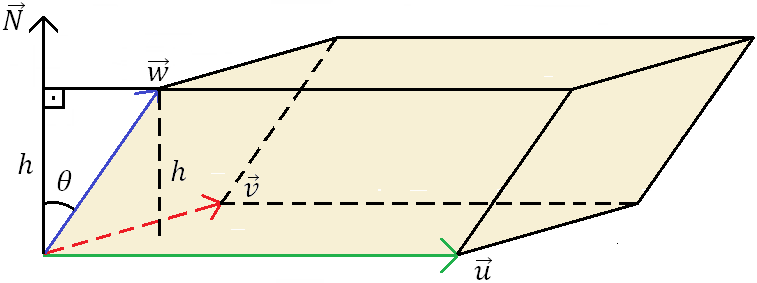
\includegraphics[width=0.4\linewidth]{analitica/imagens/misto.png}
\end{figure}

\textbf{Demonstração}: observe inicialmente que o volume do paralelepípedo é dado pela multiplicação da área da base pela altura $h$. A base é um paralelogramo determinado pelos vetores $\vec u$ e $\vec v$, cuja área é dada por $\vec u \times \vec v$. Note que a altura é dada por $h=\Vert \vec w \Vert \cdot|\cos{\theta}|$.

\begin{eqnarray*}
V & = & (\textrm{área da base})\cdot h \\
V & = & \Vert \vec u \times \vec v\Vert \cdot \Vert w\Vert\cdot |\cos{\theta}|\\
V & = & |\vec w  \cdot ( \vec u \times \vec v)|\\
V & = & |(\vec w, \vec u, \vec v )|
\end{eqnarray*}